
In this section, we give a high-level overview of our main results and the main techniques used in our  algorithms.  
 We also introduce some of the  definitions and notations along the
way; we refer the reader to~\Cref{appendix:preliminaries} and~\cite{stewart2001algebraic, StewartBook} for more details. 

\paragraph{Algebraic Circuits.}
Let $X=\{x_1,\ldots,x_k\}$ be a set of commutative variables.
An \emph{algebraic circuit}  over~$X$ is a directed acyclic graph  with labelled vertices and edges. Vertices of in-degree zero (leaves) are labelled with variables in $X$ and $-1$; and the remaining vertices have labels in $\{+,\times\}$. Moreover, the incoming edges to $+$-vertices have labels in $\mathbb{Z}$, that is, the $+$-gates compute integer-weighted sums. There is a unique vertex of out-degree zero which determines the output of the circuit, a $k$-variate polynomial, computed in an obvious bottom-up manner.
%
The \emph{size} of a circuit is the number of its gates; see Figure~\ref{fig:circuit}.
The \emph{degree} of a circuit $C$ is defined inductively as follows: input gates have degree $1$, the degree of an addition gate is the maximum of the degrees of its inputs, the degree of a multiplication gate is the sum of the degrees of its inputs, and the degree of $C$ is the degree of the output gate. Note that the degree of an algebraic circuit is an upper bound on the degree of its underlying polynomial.
Thus the total degree and the bit-length of the coefficients of a polynomial represented by a circuit is at most exponential in the size of the circuit.


\begin{figure}[t]
\begin{center}	
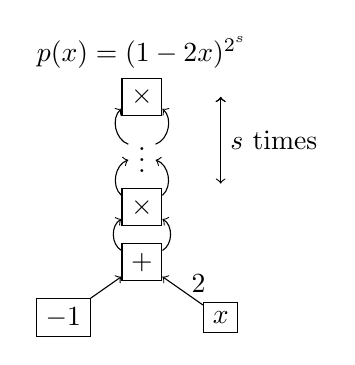
\begin{tikzpicture} 
\node[draw,label={above:$p(x)=(1-2x)^{2^s}$}] at (2,2.1) (A4) {$\times$};
 \node[draw=none] at (2,1.4) (A3) {$\vdots$};
\draw[<-,  bend left=60]  (A4) edge (A3) ;
\draw[<-,  bend right=60]  (A4) edge  (A3) ; 
  \node[draw] at (2,.7) (A2) {$\times$};
\draw[<-,  bend left=60]  (A3) edge (A2) ;
\draw[<-,  bend right=60]  (A3) edge (A2) ;   
 \node[draw] at (2,0) (A1) {$+$};
\draw[<-,  bend left=60]  (A2) edge (A1) ;
\draw[<-,  bend right=60]  (A2) edge  (A1) ; 

\node[draw] at (1,-.7) (c1) {$-1$};
\node[draw] at (3,-.7) (x) {$x$};

\draw[<-]  (A1) edge (c1) ;
\draw[<-]  (A1) edge node[near start,right]{$~2$} (x) ;
\draw[<->]  (3,2.1) edge node[midway,right]{$s$ times} (3,1) ;
 
\end{tikzpicture}
	\end{center}
	\caption{An  algebraic circuit 
	 computing   the polynomial $p(x)=(1-2x)^{2^s}$, with the highest degree monomial $x^{2^s}$ and the coefficients double exponential $2^{2^s}$ in its size~$s+3$.}\label{fig:circuit}
\end{figure}

 
\subsection{Radical Identity testing}
 

Let  $f(x_1,\ldots,x_k)$ be  a multivariate polynomial computed by an algebraic circuit, and  $\mysqrt
{d_1}{a_1},\ldots,\mysqrt{d_k}{a_k}$ be  $k$ radicals, where the radicands $a_i\in \NN$, and the exponents~$d_i\in \NN$ are nonnegative integers,  written in binary.
The \emph{Radical Identity Testing} (RIT) problem asks whether 
\[f( \mysqrt{d_1}{a_1},\ldots,\mysqrt{d_k}{a_k} )=0.\]  
We define the size of an RIT instance as the maximum of
the size of the circuit  and the bit-length of the radicands $a_i$ and exponents $d_i$.

 
\paragraph{The $2$-RIT problem.} This is a special case of RIT 
where all input radicals $\sqrt{a_1},\ldots,\sqrt{a_k}$ are square roots and all radicands $a_i$ are rational primes, written in binary.


\paragraph{The Bounded-RIT problem.}
This variant is defined exactly as the RIT problem,
except that the input also includes an upper bound on the  degree of the circuit that is given in unary. Thus in Bounded-RIT the degree of the circuit is at most the size of the instance. 


\subsection{Algebraic Number fields}

Recall that  $\alpha\in \CC$ is \emph{algebraic} if it is a root of a non-zero polynomial in $\QQ[x]$. 
The minimal polynomial of $\alpha$ (over~$\QQ$) is
the unique monic polynomial in $\QQ[x]$ (that is a polynomial with the leading coefficient~$1$) having $\alpha$ as a root.
The degree of $\alpha$ is defined to be the degree of its minimal polynomial, and denoted by $\deg \alpha$. 
 If the minimal polynomial has integer coefficients then we say that $\alpha$ is an algebraic integer.
 Given $a, d \in \NN$, the radical $\mysqrt{d}{a}$ is an algebraic integer. 
 


An \emph{algebraic number field} (or simply number field) $K$ is a finite degree field extension of~$\QQ$, that is, $K$ is a field that contains $\QQ$ and has finite dimension when considered as a vector space over $\QQ$. 
The dimension of this vector space is called the degree of the extension and is denoted by $[K:\QQ]$. We further denote by $\OO_K$  the subring of $K$ comprised by the
algebraic integers
in $K$.
The ring $\OO_K$ is a finitely generated free abelian group. 

Given $n\in \NN$, we write $\zeta_n$ for the primitive complex $n$-th root of unity $\zeta_n = e^{\frac{2\pi i}{n}}$.
The $n$-th cyclotomic polynomial, denoted by~$\Phi_n$, is the minimal polynomial of $\zeta_n$. 
The number field $\QQ(\zeta_n)$ is an extension of $\QQ$ obtained by adjoining $\zeta_n$; the degree $[\QQ(\zeta_n):\QQ]$ of the extension is the degree of $\Phi_n$. It is well known that the ring of  integers of $\QQ(\zeta_n)$ is the ring $\ZZ[\zeta_n]$
that is generated over $\ZZ$ by $\zeta_n$.

Given a polynomial $f\in \mathbb{Q}[x]$, the splitting field 
$K$ of $f$ is the subfield of $\mathbb{C}$ generated by 
the roots of $f$.  We say that a field extension $K/\mathbb{Q}$ is a Galois extension if $K$ is the splitting field of some 
polynomial.  
The Galois group of $K$ over~$\QQ$, denoted by $\Gal(K/\QQ)$, is comprised of all automorphisms of $K$ that fix $\QQ$ pointwise. The image of $\alpha \in K$ under an automorphism  $\sigma\in \Gal(K/\QQ)$ is
called a Galois conjugate of $\alpha$, in other words, the Galois conjugates of $\alpha$ are precisely all the roots of its minimal polynomial. 
The Galois conjugates of $\zeta_n$ are all its powers~$\zeta^k_n$ with $\gcd(k,n)=1$. 
The norm of $\alpha$ over a Galois extension~$K$ is defined as the product of all the Galois conjugates of $\alpha$:
\[N_{K/\QQ}(\alpha)=\prod_{\sigma\in \Gal(K/\QQ)}\sigma(\alpha).\]
Note that the norms of all Galois conjugates are equal,
and the norm of an algebraic integer is always a rational integer itself. 

The minimal polynomial of the real radical $\mysqrt{d}{a}$ over $\QQ$ has the form
$x^{t}-c$ where $t$ is the smallest positive integer such that there exists an integer $c$ with $\mysqrt{d}{a}=\mysqrt{t}{c}$.
The conjugates of $\mysqrt{d}{a}$ are then $\zeta^j_t\mysqrt{t}{c}$ with $1\leq j \leq t$.
The splitting field $K$ of
$\prod_{i=1}^k (x^{d_i}-a_i)$ is $\QQ(\mysqrt{d_1}{a_1}, \ldots, \mysqrt{d_k}{a_k},\zeta_d)$,  obtained by adjoining the radicals $\mysqrt{d_i}{a_i}$ and  a primitive root of unity $\zeta_d$, with order $d=\lcm(d_1,\ldots,d_k)$, to~$\QQ$. 


Given a number field~$K$,
the ring of integers $\OO_K$ may not be a unique factorisation domain. However we do have unique factorisation of ideals 
into products of prime ideals in $\OO_K$.  Recall here that an
ideal $\mathfrak{p} \subset \OO_k$ is called a prime ideal if for all algebraic integers $\alpha$ and $\beta$, if $\alpha\beta \in \mathfrak{p}$, then at least one of $\alpha$ and $\beta$ is in $\mathfrak{p}$. 
We say that a prime $p\in \mathbb{Z}$ splits completely in
$\OO_K$ 
if we can write $p\OO_K$ as:
\[ p\mathcal{O}_K = \mathfrak{p}_1 \cdots \mathfrak{p}_n \]
where the $\mathfrak{p}_i$ are distinct prime ideals of $\OO_K$ and $n = [K:\mathbb{Q}]$.
In the case when $K$ is the splitting field of a polynomial $f \in \mathbb{Z}[X]$
over $\mathbb{Q}$, a sufficient condition for $p$ to split completely 
over $K$ is that $f$ split into distinct linear factors over the field 
$\mathbb{Q}_p$ of $p$-adic numbers.



\subsection{Symbolic Algorithm}
Our approach to identity testing 
of algebraic numbers generalises the well-known
fingerprinting procedure for solving ACIT, which involves evaluating an arithmetic circuit modulo a randomly chosen prime. The soundness of the latter approach relies on the fact that if the integer~$z\in \ZZ$ computed by the circuit is non-zero, 
then one can with high probability randomly sample a prime $p\in \mathbb{Z}$ of size polynomial in the bit-length of the input such that $Z$ is non-zero modulo $p$. 



\bigskip
\noindent {\bf Placing RIT in \coNP:}
Given input radicals~$\mysqrt{d_1}{a_1},\ldots,$ $\mysqrt{d_k}{a_k}$ to RIT, we first reduce RIT to the case that the radicands~$a_i$ are pairwise coprime numbers and that the minimal polynomials of the input radicals $\mysqrt{d_i}{a_i}$ are $x^{d_i}-a_i$ for all $i= 1,\ldots,k$.  To do this we generalise the reduction in~\cite{blomer98} and use the \emph{factor refinement} algorithm~\cite{BACH1993199}; see \Cref{appendix:reduction}.
Denote by $K$ the splitting field  of $\prod_{i=1}^k (x^{d_i}-a_i)$.

In~\Cref{fig:conp_RIT}, we present  a conceptually simple algorithm for deciding RIT and  place this problem in {\coNP}.
Our {\coNP} procedure 
 is similar in spirit to the {\coRP}
procedure for the ACIT problem, alluded to above, inasmuch as it involves
evaluating the circuit modulo a prime ideal.
 The proof of the correctness though is not as straightforward and relies on characteristics of the Galois group of~$K$ and
 concepts from number theory. 

In the case of RIT we think of the evaluation as occurring in
the ring of integers $\mathcal{O}_K$. Specifically, the idea is to work modulo a prime ideal~$\mathfrak{p}$ of
$\mathcal{O}_K$ such that the quotient $\mathcal{O}_K / \mathfrak{p}$ is a
finite field~$\mathbb{F}_p$ for some rational prime $p$.
Note that the algorithm works directly with the finite field $\mathbb{F}_p$---the prime ideal 
$\mathfrak{p}$ is implicit in the choice of radicals in 
Line~1, and ideals in $K$ only feature in the 
proof of correctness of the algorithm.   Overall, the key idea is that 
if 
$f(\mysqrt{d_1}{a_1},\ldots,\mysqrt{d_k}{a_k}) \neq 0$
then there is a polynomial-length polynomial-time checkable witness 
of this fact --- namely
a prime~$p$ and 
$\overline{\alpha}_1,\ldots,\overline{\alpha}_k \in \mathbb{F}_p$, satisfying $\overline{\alpha}_i ^ {d_i} \equiv a_i \pmod{p}$, such that $\overline{f}(\overline{\alpha}_1,\ldots,\overline{\alpha}_k )$ is non-zero, where $\overline{f}$ is the reduction of $f$ modulo~$p$.

\begin{figure*}[t]
    \centering
    \begin{tabularx}{0.82\textwidth}{ p{0.1\textwidth} p{0.72\textwidth} }
   \rowcolor{Gray}
    \multicolumn{2}{c}{\textbf{Radical Identity Testing}} \\
    \textbf{Input:} & Algebraic circuit $C$
    of size at most $s$ with input radicals $\mysqrt{d_1}{a_1},\ldots,\mysqrt{d_k}{a_k}$ where
    the bit-length of the $d_i$ and $a_i$ is at most $s$,
    and the $a_i$ are mutually coprime. 
    \\  \rowcolor{Gray}
    \textbf{Output:} & Whether $f(\mysqrt{d_1}{a_1},\ldots,\mysqrt{d_k}{a_k})=0$ for the polynomial $f(x_1,\ldots,x_k)$ computed by $C$.
    \\  
        \textbf{Line 1:} & 
            Guess a prime $p \leq 2^{4s^3}$ and $\overline{\alpha}_1,\ldots,\overline{\alpha}_k \in \FF_p$ such that $p \equiv 1 \pmod{d}$ and $\overline{\alpha}_i^{d_i} \equiv a_i \pmod{p}$. 
    \\ 
    \textbf{Line 2:} &
            Output 'Zero' if $\overline{f}(\overline{\alpha}_1,\ldots,\overline{\alpha}_k) = 0$, where $\overline{f}$ is the reduction of $f$ modulo $p$; and 'Non-zero' otherwise.
    \\ \hline
    \end{tabularx}
    \caption{Our nondeterministic algorithm for the complement of RIT.}
    \label{fig:conp_RIT}
\end{figure*}



We first summarise the algorithm, see \Cref{fig:conp_RIT}, and then outline the correctness argument.

\begin{enumerate}
      \item We find a rational prime $p$ such that
    each polynomial among $x^{d_1}-a_1, \ldots, x^{d_k} - a_k$ splits into 
    distinct linear factors over $\mathbb{F}_p$.  We can find such a prime $p$ in non-deterministic polynomial time
    in the length of the problem instance by (i)~choosing a prime~$p$ such that $p\equiv 1 \bmod d$, which 
    ensures that $\mathbb{F}_p$ contains a primitive $d$-th root of unity,    
and (ii)~guessing and checking 
    $\overline{\alpha}_1,\ldots,\overline{\alpha}_k \in \mathbb{F}_p$ such that 
    $\overline{\alpha}_i$ is any root in $\mathbb{F}_p$ of the polynomial $x^{d_i}-a_i$.

    \item We evaluate the polynomial $\overline{f}(\overline{\alpha}_1,\ldots,\overline{\alpha}_k)$ in $\mathbb{F}_p$, where $\overline{f}(x_1,$ $\ldots,x_k) \in \mathbb{F}_p[x_1,\ldots,x_k]$ is the reduction of $f$ modulo $p$.
    If the result  of this computation is zero then we report 'Zero'; otherwise we report 'Non-zero'. 
    \end{enumerate}
    
    
    Having summarised the algorithm we can now state our main result: 
 
\begin{theorem}\label{th:rit-conp}
	The RIT problem is in {\coNP} under GRH.
\end{theorem}
    
 Below, we give a high-level idea of the correctness of~\Cref{th:rit-conp}.
   The first element of the correctness proof of the {\coNP} algorithm  is to argue that the prime $p$ chosen in Item~1 completely splits
    in the ring of integers~$\mathcal{O}_K$.
    In this situation, for any prime-ideal factor $\mathfrak{p}$ of $p$, each quotient field $\mathcal{O}_K / \mathfrak{p}$
    is isomorphic to the finite field $\mathbb{F}_p$.  
    By standard results in algebraic number theory we know that $p$ completely splits in $\mathcal{O}_K$
    if each polynomial $x^{d_1}-a_1,\ldots,x^{d_k}-a_k$ splits into linear factors over the field $\mathbb{Q}_p$ of $p$-adic numbers.
    But the latter requirement is guaranteed by Hensel's Lemma in tandem with Conditions 1(i) and 1(ii) that determine the choice of $p$ in the algorithm.
    In more detail, 
    Condition 1(i), that $p \equiv 1 \bmod d$, entails that $\mathbb{F}_p$ contains 
    a primitive $d$-th root of unity. 
Indeed, since the powers of a root of unity are also all  roots of unity themselves, and since the multiplicative group $\FF_p^{*}$ is cyclic, it is clear that $\FF_p^{*}$ contains
a primitive $d$-th root of unity just in case $d \mid p-1$. 
      In combination with Condition 1(ii), that each of the polynomials 
    $x^{d_1}-a_1, \ldots, x^{d_k} - a_k$
    has a root in $\mathbb{F}_p$, we can conclude that
    each of the above polynomials in fact splits into distinct linear factors over $\mathbb{F}_p$.
    Then Hensel's Lemma allows us to lift this factorisation over $\mathbb{F}_p$ into a factorisation 
    into distinct linear factors over $\mathbb{Q}_p$.
    

    
    The second element of the correctness proof concerns the choice of 
    $\overline{\alpha}_1,\ldots,\overline{\alpha}_k$ in $\mathbb{F}_p$.   In particular,
    we argue that the correctness of the algorithm does not rely, for $i=1,\ldots,k$, on a specific choice of $\overline{\alpha}_i$
    among the $d_i$ roots of $x^{d_i} - a_i$ in $\mathbb{F}_p$.  This argument is based on the fact
    that the Galois group
    $\mathrm{Gal}(K / \mathbb{Q})$ acts transitively on the set 
    \[ \{ (\alpha_1,\ldots,\alpha_k) \in K^k : \alpha_1^{d_1}=a_1 \wedge \cdots \wedge \alpha_k^{d_k} = a_k \} \]
   	   	 That is, for any two $k$-tuples $\tau_1$ and $\tau_2$ in the set above, there exists an automorphism $g$ in $\Gal(K/\QQ)$ such that $g(\tau_1) = \tau_2$.
    We will call this property joint transitivity; see \Cref{lem:jtrans}.
 
 
     Now for every prime ideal factor $\mathfrak{p}$ of $p\mathcal{O}_K$ there is a
surjective homomorphism $\varphi: \mathcal{O}_K \rightarrow \mathbb{F}_p$ with kernel
$\mathfrak{p}$.   For each choice of $\mathfrak{p}$ and for all $i=1,\ldots,k$, the corresponding homomorphism 
$\varphi$ maps $\alpha_i$ to some root $\overline{\alpha}_i$ of $x^{d_i} - a_i$ in $\mathbb{F}_p$.
Conversely, using joint transitivity, we are able to show that every
mapping $\alpha_1 \mapsto \overline{\alpha}_1, \ldots, \alpha_k \mapsto \overline{\alpha}_k$
where, for $i=1,\ldots,k$, $\overline{\alpha}_i$ is an arbitrary root of $x^{d_i} - a_i$ in $\mathbb{F}_p$,
arises from the quotient map by some prime ideal factor of $p$.
We conclude that the value $\overline{f}(\overline{\alpha}_1,\ldots,\overline{\alpha}_k)$ in Item 2 is 
the image of $f(\alpha_1,\ldots,\alpha_k)$ under the quotient map $\OO_K \to \OO_K / \mathfrak{p}$ for some prime ideal $\mathfrak{p}$.
    
    It follows from the line immediately above that
    the algorithm has no false positives: if $f(\alpha_1,\ldots,\alpha_k)=0$ in $K$ then certainly 
    $\overline{f}(\overline{\alpha}_1,\ldots,\overline{\alpha}_k)= 0$.
    We moreover show that for a suitable choice of prime $p$, namely such that $p$ does not
    divide the norm of~$f(\alpha_1,\ldots,\alpha_k)$ over $K/\mathbb{Q}$,
    the converse holds:
    if $f(\alpha_1,\ldots,\alpha_k)\neq 0$ in $K$
    then
    $\overline{f}(\overline{\alpha}_1,\ldots,\overline{\alpha}_k)\neq 0$
    in $\mathbb{F}_p$.
For more details, see \Cref{th:RIT-soundess}.

A quantitative version of the Chebotarev density theorem
guarantees that we can find such a prime of polynomial bit-length that splits.
Informally speaking, Chebotarev's density theorem states that the set of rational primes $p$ that split completely in $\OO_K$ has density $\frac{1}{|\Gal(K/\QQ)|}$.
The original statement of the theorem~\cite{Stevenhagen95chebotarevand}
is asymptotic, whereas for our algorithm we use its quantitative version in order to obtain a bound on the number of primes $p$ of size polynomial in the bit-length of the input such that $p\OO_K$ completely splits, which requires GRH~\cite{lagariasO, serre1981quelques}.
We use the bound in combination with a bound on the norm of $f(\alpha_1,\ldots,\alpha_k)$ to ensure we can find at least one small prime that will not divide the norm and ensure our computation is sound.


\bigskip
\noindent {\bf Placing $2$-RIT in {\coRP}:}
%
We improve the obtained {\coNP} bound for  RIT  in the case of $2$-RIT, wherein all input radicals are square roots and all radicands $a_i$ are 
rational odd primes
(written in binary).
We show that $2$-RIT is in {\coRP} under GRH, and that it is in {\coNP} unconditionally.
Our {\coRP} algorithm  chooses a suitable random prime to be used in the symbolic computation. 
As discussed above,  the natural density of such suitable primes is $\frac{1}{|\Gal(K/\QQ)|}$, which is not  sufficient even for $2$-RIT.  However, we show that there is an arithmetic progression with a good density of primes, and that all primes in this progression are suitable.
To obtain this result, we rely on the law of quadratic reciprocity, as well as Dirichlet’s theorem on the density of primes in arithmetic progressions. 


We recall that a suitable  prime $p$ for our symbolic algorithm  is  such that 
the minimal polynomials of all input radicals split into linear factors over~$\FF_p$. In the setting of $2$-RIT, the minimal polynomials of the inputs are in the form $x^2-q_i$ where $q_i$ is a rational prime. The above requires that the equations $x^2 \equiv q_i$ have  solutions in $\FF_p$, that is, $q_i$ is a quadratic residue modulo~$p$. 
%
But then by the law of quadratic reciprocity, $p$ is a quadratic residue modulo prime $q_i$ if and only if $q_i$ is a quadratic residue modulo~$p$, condition to  $p \equiv 1 \pmod{4}$. 
Roughly speaking, the latter holds if $p \equiv 1 \pmod{4q_i}$ (as $1$ is a perfect square in $\FF_p$). 

By the Chinese remainder theorem and a more detailed argument similar to the above, 
we show 
that there is an arithmetic progression $A\NN+b$ such that 
for all primes $p$ in the progression, all  polynomials 
$x^2-q_i$, with $i\in \{1,\cdots,k\}$, split into linear factors over~$\FF_p$. 
We further impose another
condition on $A$
and $b$, based on Pocklington's algorithm, such that 
a root of each $x^2-q_i$ can be computed in deterministic polynomial time in the length of the problem instance.   

Finally, 
we use  estimates on the density of primes in an arithmetic
progression, see~\Cref{th:prime_density}, to obtain the following result:

\begin{theorem}\label{th:squareRIT-coRP}
The $2$-RIT problem is in {\coRP} assuming GRH and in {\coNP} unconditionally.
\end{theorem}

